\documentclass[12pt]{article} % The document class with options

\usepackage[margin=1in]{geometry}
\usepackage[utf8]{inputenc} 
\geometry{a4paper}
\usepackage{newtxtext,newtxmath}
\usepackage[T1]{fontenc}
\usepackage{amsmath}
\usepackage{amsfonts}
\usepackage{microtype}
\usepackage{graphicx}
\usepackage{listings} % For formatting and highlighting code
\usepackage{color}    % For colors in code highlighting

% Define colors for syntax highlighting
\usepackage{color}
\definecolor{dkgreen}{rgb}{0,0.6,0}
\definecolor{gray}{rgb}{0.5,0.5,0.5}
\definecolor{mauve}{rgb}{0.58,0,0.82}

% Code listing style named "mystyle"
\lstset{frame=tb,
  language=Python,
  aboveskip=3mm,
  belowskip=3mm,
  showstringspaces=false,
  columns=flexible,
  basicstyle={\small\ttfamily},
  numbers=none,
  numberstyle=\tiny\color{gray},
  keywordstyle=\color{blue},
  commentstyle=\color{dkgreen},
  stringstyle=\color{mauve},
  breaklines=true,
  breakatwhitespace=true,
  tabsize=3
}
% chktex-file 3
% chktex-file 8
% chktex-file 10
% chktex-file 17
% chktex-file 18
% chktex-file 36
% chktex-file 44

\begin{document}
\setlength{\parskip}{1em} 
\setlength{\parindent}{0pt}
\newcommand{\vect}[1]{\mathbf{#1}}

\begin{titlepage}  % This starts a title page environment
    \centering    % Center everything on the page

    %--- Add space at the top of the page ---
    \vspace*{2cm}
    
    %--- Title ---
    \normalsize \textbf{MECH 503 Final Exam} \\

  
    \vspace{2cm}  % Space between the title and the author name
    
    %--- Author ---
    \normalsize by\\
    \vspace{1cm}
    \normalsize Jincong Li \\ 
    \vspace{1cm}
    \normalsize M.Eng, The University of British Columbia, 2024
    \vspace{11cm}  % Space between the author and the date
    
    %--- Date ---
    \normalsize \today

    \vfill  % Push the following content to the bottom of the page
    %--- Bottom part of the page ---
    © Jincong Li, 2024
\end{titlepage}
\tableofcontents
\newpage
\section{Question 1}
\begin{align*}
    BC_1 &= \sigma_{xy}(x,y=\pm \frac{h}{2}) = 0\\
    BC_2 &= \sigma_{y}(x,y=\frac{h}{2}) = 0\\
    BC_3 &= \sigma_{y}(x,y=\frac{-h}{2}) = -q\\
    BC_4 &= \int_{\frac{-h}{2}}^{\frac{h}{2}} \sigma_x(x=\pm L,y) = 0 \\
    BC_5 &= \int_{\frac{-h}{2}}^{\frac{h}{2}} \sigma_x(x=\pm L,y)y = 0 \\
    BC_6 &= \int_{\frac{-h}{2}}^{\frac{h}{2}} \sigma_{xy}(x=\pm L,y) = \pm Lq \\
\end{align*}
One could observe the boundary conditions are satisfied in classical and weak sense. For the normal stress in x-direction:
\[ \sigma_x(x=\pm L,y) = \pm \frac{q y \left(3 h^{2} - 20 y^{2}\right)}{5 h^{3}} \] which is symmetric about the y-axis, thus, the moment is balanced.
\begin{figure}[ht]
    \centering
    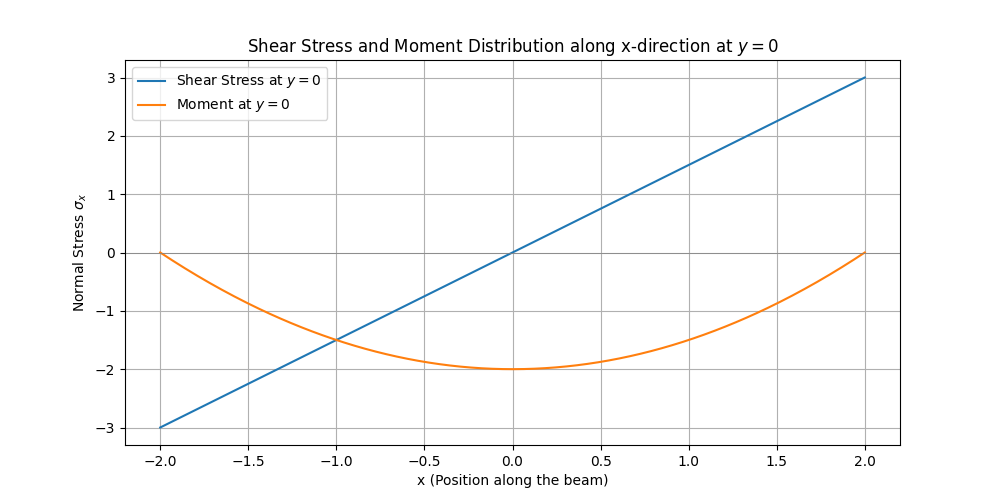
\includegraphics[width=1\textwidth]{Q1.png}
    \caption{Shear Stress and Moment Distribution along x-direction at $y=0$}
\end{figure}
The distribution of shear stress and moment is shown in figure 1, since no specific property values are given, one could conclude
that the general shape of the distribution agrees with the theory.

The Python code is provided in the Appendix file.

\section{Question 2}
\subsection*{Part 1}
\begin{align*}
    \sigma_{\theta\theta}(r=a) &= 0\\
    \sigma_{r\theta}(r=a) &= 0\\
\end{align*}
\subsection*{Part 2}
\begin{align*}
    \sigma_{rr}(\frac{r}{a}=\infty ) &= \sigma_{0} \sin^{2}{\left(\theta \right)}\\
    \sigma_{r\theta}(\frac{r}{a}=\infty ) &= - \frac{\sigma_{0} \sin{\left(2 \theta \right)}}{2}\\
    \sigma_{\theta\theta}(\frac{r}{a}=\infty ) &= \sigma_{0} \sin^{2}{\left(\theta \right)}\\
\end{align*}
\subsection*{Part 3}
\begin{align*}
    \sigma_{xx}(\frac{r}{a}=\infty ) &= - \sigma_{0} \sin^{2}{\left(\theta \right)} \cos{\left(2 \theta \right)}\\
    \sigma_{yy}(\frac{r}{a}=\infty ) &= - \frac{\sigma_{0} \sin{\left(4 \theta \right)}}{4}\\
    \sigma_{xy}(\frac{r}{a}=\infty ) &= - \sigma_{0} \sin^{2}{\left(\theta \right)} \cos{\left(2 \theta \right)}\\
\end{align*}
\newpage
\subsection*{Part 4}
\begin{figure}[ht]
    \centering
    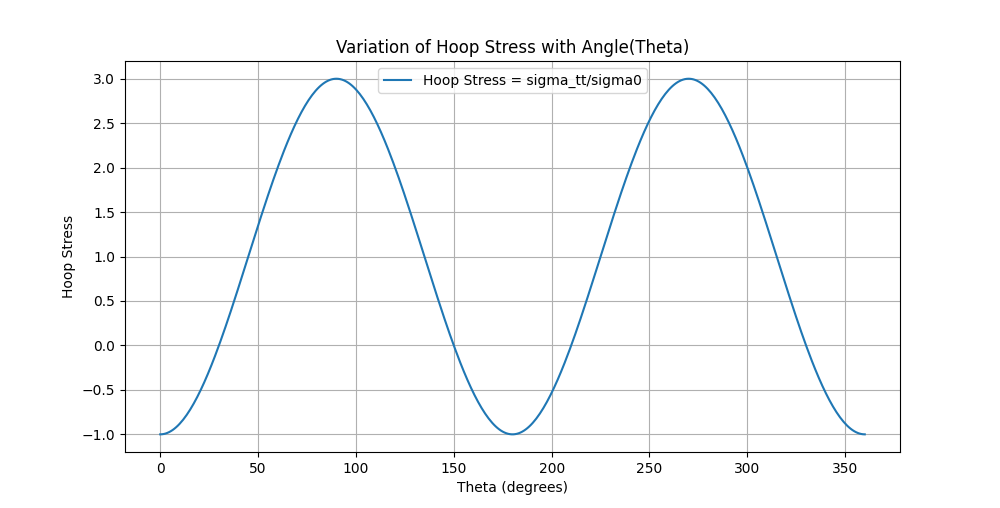
\includegraphics[width=1\textwidth]{Hoop Stress.png}
    \caption{Hoop Stress vs. Angle($\theta$)}
\end{figure}
The maximum value of hoop stress is 3, which occurs at $\theta$ = 90.0 degrees.
\subsection{Part 5}
\begin{figure}[ht]
    \centering
    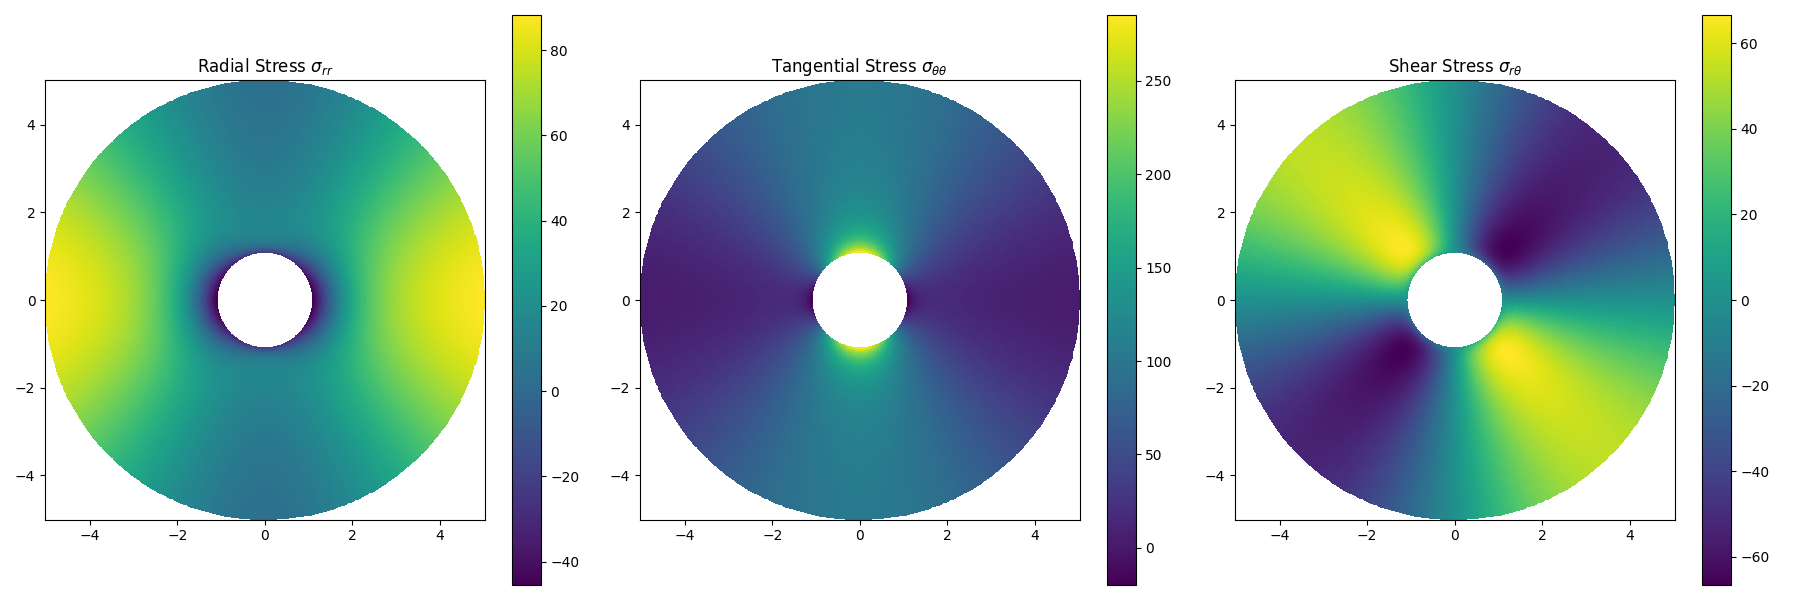
\includegraphics[width=1\textwidth]{Q2.png}
    \caption{Stress Distribution around the Hole}
\end{figure}
The radius is assumed to be 1m which is different from the given value, however, the general idea is the same.
\section{Question 3}
\subsection{Part A}
By equilibrium equation and divergence theorem:
\begin{align*}
    \rho \frac{\partial^2 u_i}{\partial t^2} &= \sigma_{ij,j}
\end{align*}
The stress tensor is given by:
\[
\sigma_{ij} = C_{ijkl} \epsilon_{kl}
\]
where \(C_{ijkl}\) are the elastic stiffness coefficients, and the infinitesimal strain tensor is given by:
\[
\epsilon_{kl} = \frac{1}{2} (u_{k,l} + u_{l,k})
\]

Substituting:
\[
\sigma_{ij,j} = (C_{ijkl} \epsilon_{kl})_{,j} = C_{ijkl} \epsilon_{kl,j}
\]
Since \(C_{ijkl}\) are constants with respect to spatial coordinates:
\[
\sigma_{ij,j} = C_{ijkl} \frac{1}{2} (u_{k,lj} + u_{l,kj})
\]


Since \(C_{ijkl} = C_{ijlk}\) and the first equation,
\[
C_{ijkl} u_{k,lj} = \rho \frac{\partial^2 u_i}{\partial t^2}
\]

\[
\rho \frac{\partial^2 u_i}{\partial t^2} = C_{ijkl} \frac{\partial^2 u_k}{\partial x_j \partial x_l}
\]

\subsection{Part b}

\begin{align*}
u_i &= a_i \exp[i \omega (t - \frac{x_j p_j}{c})] \\
u_{i,j} &= -\frac{i \omega p_j}{c} a_i \exp[i \omega (t - \frac{x_j p_j}{c})]\\
u_{i,jk} &= -\frac{i \omega p_j}{c} (-\frac{i \omega p_k}{c}) a_i \exp[i \omega (t - \frac{x_j p_j}{c})] \\
&= \frac{\omega^2}{c^2} p_j p_k a_i \exp[i \omega (t - \frac{x_j p_j}{c})]\\
C_{ijkl} \frac{\omega^2}{c^2} p_l p_k a_k \exp[i \omega (t - \frac{x_j p_j}{c})] &= \rho \omega^2 a_i \exp[i \omega (t - \frac{x_j p_j}{c})]\\
C_{ijkl} p_l p_k a_k &= \rho c^2 a_i
\end{align*}
This last equation states that the product of \(C_{ijkl}\) with \(p_l p_k\) must equal \(\rho c^2\) times the identity matrix when contracted with \(a_k\). This implies that \(a_i\) and \(p_i\) must be eigenvectors of the tensor equation, with \(c^2\) being related to the corresponding eigenvalue. This shows that a plane wave solution is feasible under certain conditions on the wave vector \(p_i\), frequency \(\omega\), and phase velocity \(c\).


\section{Question 4}
This question in coded in Python entirely, thus, for detail information, please refer to the code provided in Appendix file.
And also note that the computation process is modified according to the MATLAB code posted on Canvas. Mode 1 here is the speed in longitudinal and mode 2\&3 are the speed in shear.
\begin{figure}[ht]
    \centering
    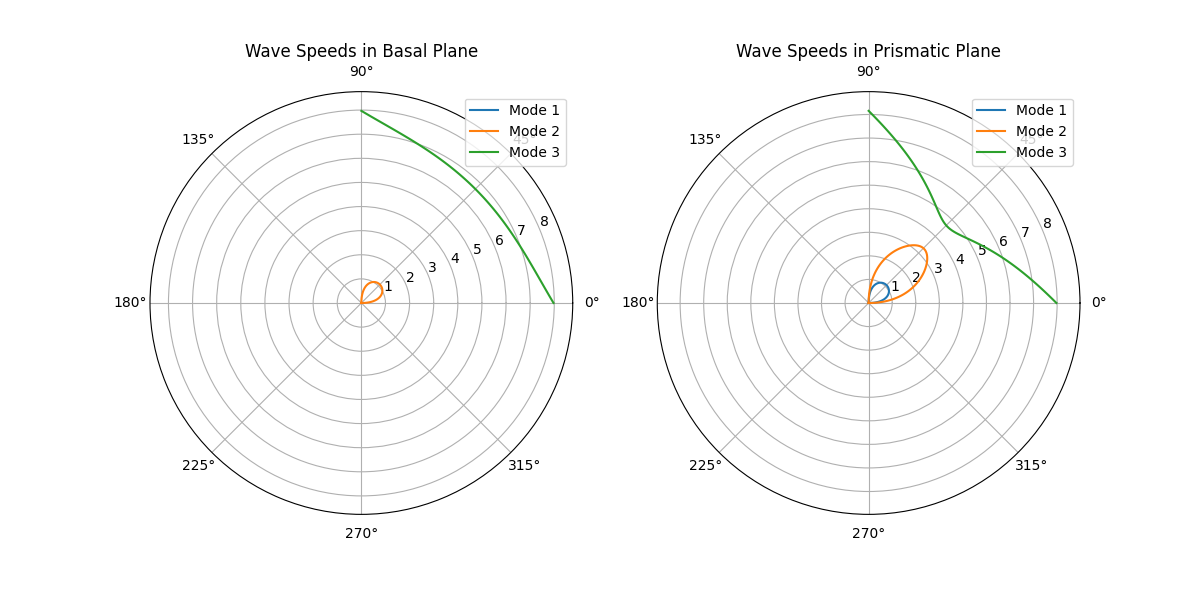
\includegraphics[width=0.8\textwidth]{Q4.png}
    \caption{Wave Speed Distribution in Polar Plot}
\end{figure}

\clearpage
\section{Question 5}
\section{Question 6}

\end{document}